% use paper, or submit
% use 11 pt (preferred), 12 pt, or 10 pt only

\documentclass[letterpaper, preprint, paper,11pt]{AAS}	% for preprint proceedings
%\documentclass[letterpaper, paper,11pt]{AAS}		% for final proceedings (20-page limit)
%\documentclass[letterpaper, paper,12pt]{AAS}		% for final proceedings (20-page limit)
%\documentclass[letterpaper, paper,10pt]{AAS}		% for final proceedings (20-page limit)
%\documentclass[letterpaper, submit]{AAS}			% to submit to JAS

\usepackage{bm}
\usepackage{amsmath}
\usepackage{subfigure}
%\usepackage[notref,notcite]{showkeys}  % use this to temporarily show labels
\usepackage[colorlinks=true, pdfstartview=FitV, linkcolor=black, citecolor= black, urlcolor= black]{hyperref}
\usepackage{overcite}
\usepackage{footnpag}			      	% make footnote symbols restart on each page
\usepackage{tikz}
\usetikzlibrary{shapes.geometric, arrows.meta, positioning}

\tikzstyle{process} = [rectangle, minimum width=3.5cm, minimum height=1cm, text centered, draw=black, fill=blue!10]
\tikzstyle{decision} = [diamond, minimum width=3cm, minimum height=1cm, text centered, draw=black, fill=yellow!20]
\tikzstyle{startstop} = [ellipse, minimum width=3cm, text centered, draw=black, fill=red!20]
\tikzstyle{arrow} = [thick, ->, >=stealth]

\PaperNumber{XX-XXX}

\begin{document}

\title{Advanced Modeling Techniques for Analyzing Space Debris Fragmentation and Evolution}

\author{Juan F Puerta-Ibarra\thanks{Professor, Department of Mechanical and Aerospace Engineering, Universidad de Antioquia, calle 67 No. 53 - 108, Medellín - Colombia},  
Bonnie Prado Pino\thanks{Adjunct Professor, Department of Mechanical and Aerospace Engineering, Universidad de Antioquia, calle 67 No. 53 - 108, Medellín - Colombia. Design Engineer, Odyssey Space Research, Houston, TX 77058},
\ and Nicolas Muñoz-Galeano \thanks{Professor, Research Group in Efficient Energy Management (GIMEL), Department of Electrical Engineering, Universidad de Antioquia, calle 67 No. 53 - 108, Medellín - Colombia}
}

\maketitle{} 		

\begin{abstract}
The increasing presence of space debris poses significant challenges to orbital sustainability, necessitating advanced modeling techniques for long-term analysis. This research presents a computational framework for analyzing the evolution of debris generated by object fragmentation in orbit, incorporating realistic debris scenarios. The framework enables forward and backward propagations utilizing N-body\cite{tamayo_reboundx_2020} symplectic integrators, facilitating a comprehensive assessment of collision risks and debris evolution. The study examines long-term population dynamics across various orbital regimes, evaluating the accuracy of symplectic methods in complex fragmentation environments. This approach enhances understanding of orbital debris and informs mitigation strategies for sustainable space operations.
\end{abstract}

\section{Introduction}
Fragmentation of space debris is a critical issue in the context of increasing space activities and the sustainability of the orbital environment. Since the dawn of the space age, the number of artificial objects in orbit has grown significantly, with estimates indicating over 31,000 objects larger than 10 cm and approximately 500,000 objects larger than 1 cm currently in low Earth orbit (LEO)\cite{pastor_early_2023}. Fragmentation events, which can occur due to collisions, explosions, or structural failures, contribute substantially to the debris population\cite{francesconi_cst_2019}. The intentional destruction of satellites and accidental fragmentation events and collisions have generated a significant portion of the debris, with catastrophic events leading to thousands of fragments\cite{noauthor_esas_nodate}. The Kessler syndrome, a scenario in which the density of objects in LEO becomes so high that collisions become inevitable, underscores the urgency of addressing fragmentation and its implications for operational spacecraft\cite{kessler_environment_1985}.

The dynamics of space debris fragmentation are complex and influenced by various factors, including the physical properties of the objects involved and their quantities, the nature of the fragmentation event, and the orbital environment. Fragmentation models, such as the NASA Standard Breakup Model\cite{johnson_nasas_2001}, provide a framework for understanding the size and velocity distributions of debris generated during such events. These models have evolved over the years, incorporating data from ground tests and on-orbit events to improve their predictive capabilities. The challenge lies in accurately modeling the fragmentation process, as the resulting debris can vary widely in size and behavior, complicating the assessment of collision risks and the long-term evolution of the debris environment.

%\begin{figure}
%    \centering
%    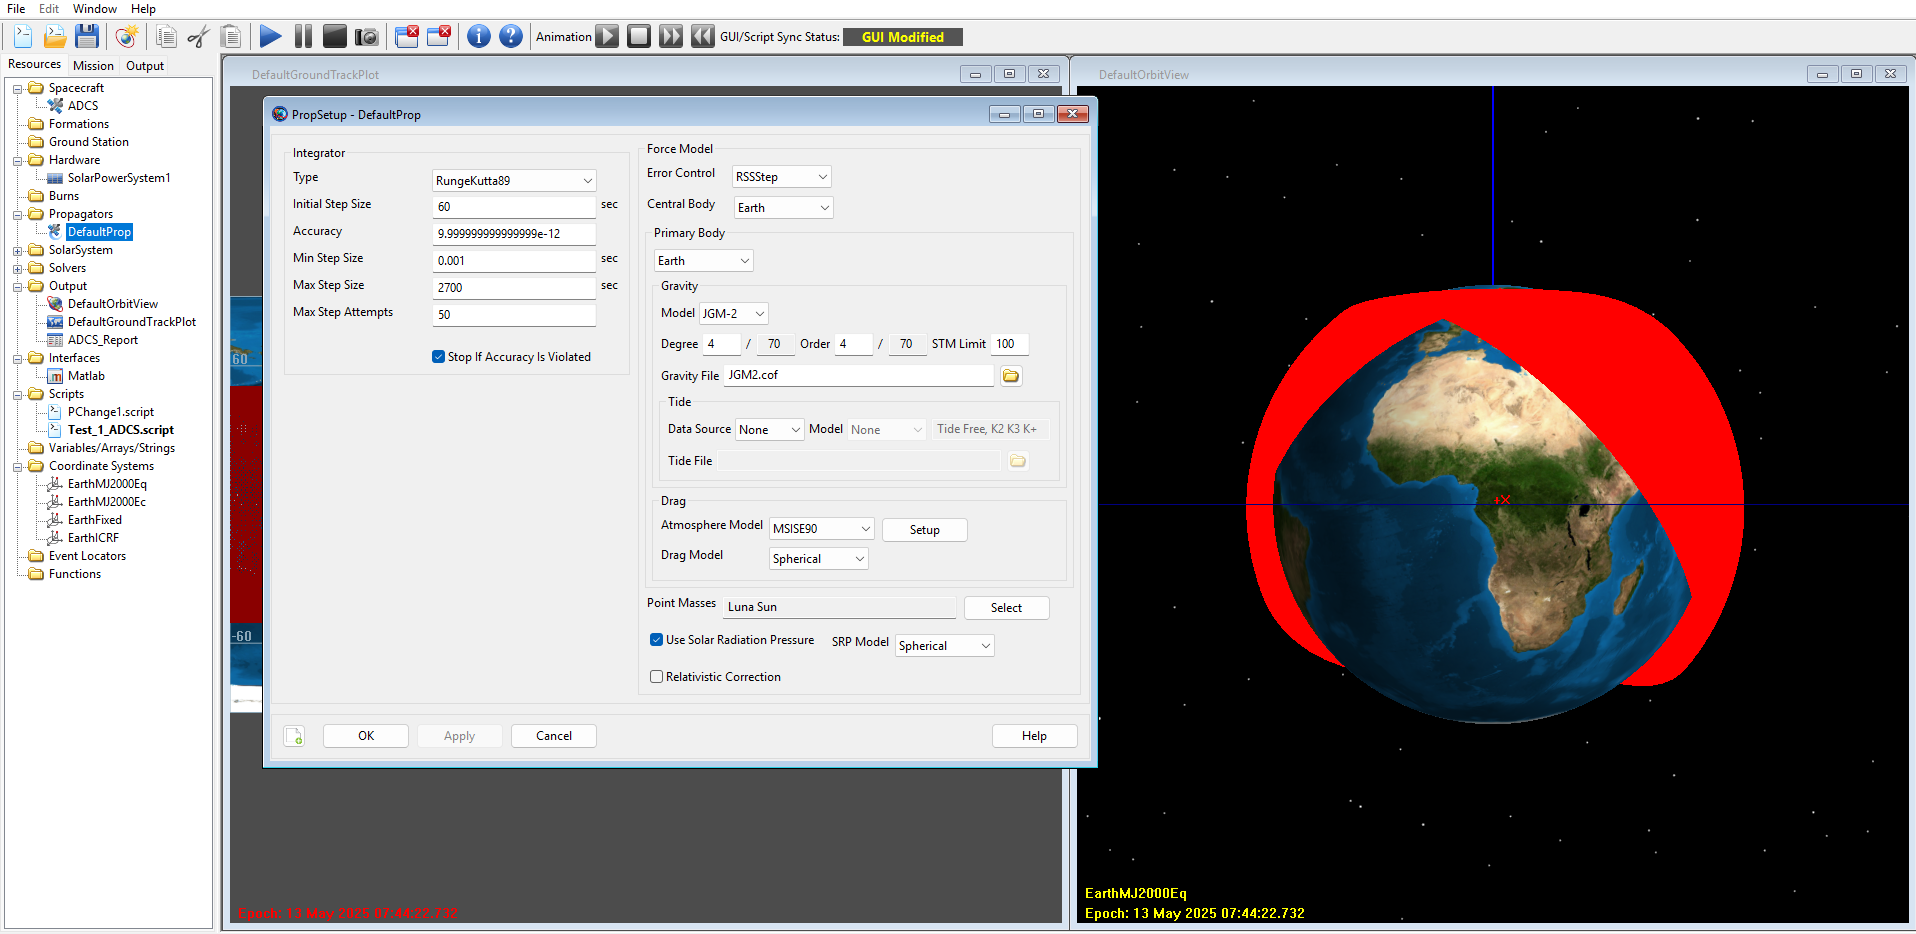
\includegraphics[width=1\linewidth]{GMAT_AIAA.png}
%    \caption{NASA's General Mission and Analysis Tool (GMAT) propagation methods}
%    \label{GMAT}
%\end{figure}

\section{Traditional Propagation Methods}
Multibody orbit propagation is essential for analyzing the trajectories of both intact satellites and fragments resulting from fragmentation events. Traditional methods often focus on larger debris objects, neglecting the significant contribution of smaller fragments to collision probabilities. One of the most widely used traditional techniques for propagating two-body orbits is \textit{Cowell’s method}, which directly integrates the equations of motion by summing all gravitational and non-gravitational forces acting on the object. This method treats the object’s acceleration as a vector derived from the central body attraction and perturbing forces, such as atmospheric drag, solar radiation pressure (SRP), and third-body effects. The integration is typically performed using standard numerical schemes like Runge-Kutta or multistep methods. While Cowell’s approach is straightforward and flexible, it is also sensitive to numerical errors, especially in long-term simulations, due to the accumulation of truncation and round-off errors.

Cowell’s method integrates Newton’s second law directly:

\begin{equation}
\ddot{\mathbf{r}} = \mathbf{a}_{\text{grav}} + \sum_{i} \mathbf{a}_{i}
\end{equation}

Where:

\begin{itemize}
    \item $\mathbf{r}$ is the position vector of the satellite,
    \item $\mathbf{a}_{\text{grav}}$ is the central body gravitational acceleration,
    \begin{equation}
        \mathbf{a}_{\text{grav}} = -\frac{\mu}{r^3} \mathbf{r}
    \end{equation}
    \item $\mathbf{a}_{i}$ represents all perturbative accelerations (e.g., atmospheric drag, solar radiation pressure, third-body effects, etc.).
\end{itemize}

An alternative to Cowell’s formulation for propagating Keplerian orbits is \textit{Encke’s method}, which focuses on integrating the deviation of a perturbed orbit from a known reference orbit. Instead of computing the full trajectory from scratch, Encke’s method calculates the difference between the real orbit and the osculating elements of the reference trajectory. This differential approach improves numerical stability, particularly when dealing with small perturbations. It also allows for more efficient integration, as the main gravitational influence is analytically accounted for in the reference solution, reducing the computational load of recalculating dominant forces at every step.

Encke’s method integrates the deviation $\boldsymbol{\rho}=\mathbf{r}-\mathbf{r_0}$ from a reference orbit $\mathbf{r_0(t)}$:

\begin{equation}
\ddot{\boldsymbol{\rho}} = \mathbf{a}(\mathbf{r}_0 + \boldsymbol{\rho}) - \mathbf{a}_0(\mathbf{r}_0) - \ddot{\mathbf{r}}_0
\end{equation}

Where

\begin{itemize}
    \item $\boldsymbol{\rho}$ is the deviation vector.
    \item $\mathbf{a}(\mathbf{r}_0 + \boldsymbol{\rho})$ is the total acceleration at the true position,
    \item $\mathbf{a}_0(\mathbf{r}_0)$ is the nominal central force,
    \item $\ddot{\mathbf{r}}_0$ is the acceleration of the reference orbit.
\end{itemize}

Another classical technique is the method of variation of parameters, also known as \textit{Gauss’ method}. This method reformulates the problem in terms of time-varying orbital elements, rather than Cartesian position and velocity vectors. By applying Gauss’ planetary equations, the evolution of orbital parameters due to perturbations can be directly computed. This approach offers valuable insights into the physical mechanisms driving orbital changes, such as secular drifts or periodic variations. It is particularly useful for analyzing the long-term effects of specific perturbing forces, though it may be less suitable for orbits undergoing frequent or abrupt changes.\cite{montenbruck_satellite_2000}. 

The method uses the Gauss planetary equations to describe the time derivatives of the orbital elements $(a,e,i,\Omega,\omega,\nu)$. For instance, the time derivative of the semi-major axis $a$ under perturbing accelerations $(R,T,N)$ in the radial, transverse, and normal directions is:

\begin{equation}
\frac{da}{dt} = \frac{2}{n \sqrt{1 - e^2}} \left[ e R \sin \nu + \frac{p}{r} T \right]
\end{equation}

Where:

\begin{itemize}
    \item $n$ is the mean motion,
    \item $p=1-e^2$ is the semi-latus rectum,
    \item $\nu$ is the true anomaly
\end{itemize}

In contrast to the traditional propagation methods discussed in this section, symplectic integrators have been adopted in celestial mechanics due to their structure-preserving properties, particularly for Hamiltonian systems governed by conservative forces. Their ability to conserve phase-space volume and exhibit bounded energy error over long periods makes them ideal for multibody dynamics and high precision orbit propagation\cite{hubaux_symplectic_2012}.


\section{Symplectic Propagation Methods}
This research seeks to advance the modeling of orbital debris evolution by investigating the long-term behavior of fragmented spacecraft populations under the influence of multibody gravitational dynamics and non-conservative forces. The main objective is to develop and extend the applicability of symplectic orbit propagators to environments such as LEO, where dissipative forces—primarily atmospheric drag and SRP play a significant role.

While symplectic integrators are well-established in preserving energy and phase-space structure in conservative systems, their use in space applied missions and scenarios involving energy dissipation remains an open area of research. By integrating fragmentation models with N-body symplectic propagation methods, this study aims to construct a computational framework capable of simulating the forward and backward evolution of debris fields, assessing collision risk, and analyzing population growth over decades to centuries.

This work explores how these methods can improve the prediction accuracy and computational efficiency in modeling debris evolution, and quantify the impact of long-term debris propagation on the stability and sustainability of orbital environments, particularly with conservative and non-conservative forces. Ultimately, the research contributes to improve debris risk forecasting and provides insight for space traffic management and sustainability policy development.

\subsection{Overview of Symplectic Methods Applied to Orbital Mechanics}

This research develops a semi-symplectic integration approach that enables the long-term propagation of objects (active and non-active) in low Earth orbit, accounting for both conservative and non-conservative forces. The method splits the forces acting on the spacecraft into two distinct types: a Hamiltonian (conservative) gravitational component and a perturbative component that includes atmospheric drag and SRP. The framework is based on second-order symplectic splitting techniques with Extended Phase Space/Splitting Methods such as Lie-Trotter or Strang splitting, ensuring accuracy and numerical stability over long propagation times\cite{luo_applying_2017}. In general, the motion is governed by the second-order ordinary differential equation:

\begin{equation}
    \frac{dv}{dt} = \bm{a}_{\text{grav}} + \bm{a}_{\text{drag}} + \bm{a}_{\text{SRP}}
\end{equation}

where $v$ is the velocity vector, and the terms on the right-hand side represent the respective accelerations due to gravity, atmospheric drag, and SRP.

The gravitational acceleration is modeled as:
\begin{equation}
    \bm{a}_{\text{grav}} = -\frac{\mu}{r^3} \bm{r}
\end{equation}

Atmospheric drag is treated as a non-conservative force, defined by:

\begin{equation}
    \bm{a}_{\text{drag}} = -\frac{1}{2} \frac{C_D A}{m} \rho(v) \, v \, \bm{v}
\end{equation}
where:
\begin{itemize}
    \item $C_D$ is the drag coefficient,
    \item $A$ is the cross-sectional area,
    \item $m$ is the object mass,
    \item $\rho(v)$ is the atmospheric density.
\end{itemize}

SRP, a non-conservative force, is represented by:

\begin{equation}
    \bm{a}_{\text{SRP}} = -P_{\text{SRP}} \frac{A_{\text{SRP}}}{m} (1 + q) \, \hat{\bm{r}}_{\text{sun}}
\end{equation}
where:
\begin{itemize}
    \item $P_{\text{SRP}}$ is the solar radiation pressure,
    \item $A_{\text{SRP}}$ is the effective SRP area,
    \item $q$ is the reflectivity coefficient,
    \item $\hat{\bm{r}}_{\text{sun}}$ is the unit vector from the satellite to the Sun.
\end{itemize}

\subsection{Lie–Trotter and Strang splitting formulations}

The integration of orbital dynamics influenced by both conservative and non-conservative forces can be approached using operator splitting techniques. In this context, the total evolution operator $\Phi(\Delta t)$ is decomposed into two components: $\Phi_G$, which represents the exact or numerically accurate flow of the gravity-only system (e.g., solved via symplectic leapfrog or Kepler solver), and $\Phi_P$, which accounts for perturbative forces such as atmospheric drag and solar radiation pressure. The Lie–Trotter splitting scheme applies the perturbation and gravitational flows sequentially as $\Phi_P(\Delta t) \circ \Phi_G(\Delta t)$, while the more accurate second-order Strang splitting applies the perturbative flow in symmetric half-steps:

\begin{equation}
    \Phi(\Delta t) \approx \Phi_P\left(\frac{\Delta t}{2}\right) \circ \Phi_G(\Delta t) \circ \Phi_P\left(\frac{\Delta t}{2}\right)
\end{equation}

Figure~\ref{fig:strang_splitting_flow} shows a graphical representation of this framework, where the perturbation flow $\Phi_P$ is not integrated via a symplectic method, but instead it is applied as a direct correction to the satellite's velocity vector. The perturbation step updates the velocity according to:

\begin{equation}
    \bm{v} \leftarrow \bm{v} + \Delta t \cdot \left( \bm{a}_{\text{drag}} + \bm{a}_{\text{SRP}} \right)
\end{equation}

\begin{figure}[htbp]
    \centering
    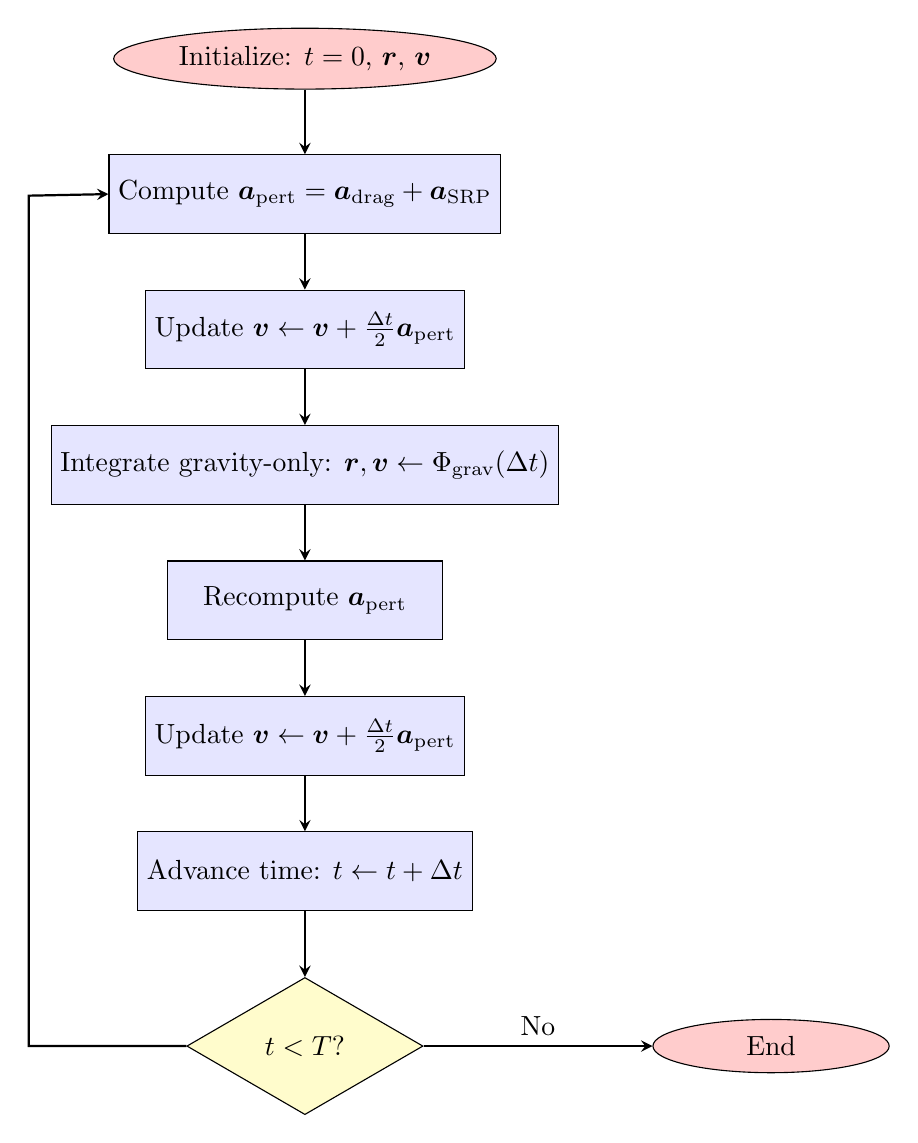
\begin{tikzpicture}[node distance=1.72 cm]
    % Nodes
    \node (start) [startstop] {Initialize: $t = 0$, $\bm{r}$, $\bm{v}$};
    \node (a1) [process, below of=start] {Compute $\bm{a}_{\text{pert}} = \bm{a}_{\text{drag}} + \bm{a}_{\text{SRP}}$};
    \node (a2) [process, below of=a1] {Update $\bm{v} \leftarrow \bm{v} + \frac{\Delta t}{2} \bm{a}_{\text{pert}}$};
    \node (a3) [process, below of=a2] {Integrate gravity-only: $\bm{r}, \bm{v} \leftarrow \Phi_{\text{grav}}(\Delta t)$};
    \node (a4) [process, below of=a3] {Recompute $\bm{a}_{\text{pert}}$};
    \node (a5) [process, below of=a4] {Update $\bm{v} \leftarrow \bm{v} + \frac{\Delta t}{2} \bm{a}_{\text{pert}}$};
    \node (a6) [process, below of=a5] {Advance time: $t \leftarrow t + \Delta t$};
    \node (decide) [decision, below of=a6, yshift=-0.5cm] {$t < T$?};
    \node (stop) [startstop, right of=decide, xshift=4.2cm] {End};
    
    % Arrows
    \draw [arrow] (start) -- (a1);
    \draw [arrow] (a1) -- (a2);
    \draw [arrow] (a2) -- (a3); 
    \draw [arrow] (a3) -- (a4);
    \draw [arrow] (a4) -- (a5);
    \draw [arrow] (a5) -- (a6);
    \draw [arrow] (a6) -- (decide);
    \draw [arrow] (decide) -- node[above] {No} (stop);
    \draw [arrow] (decide.west) -- ++(-2,0) -- ++(0,10.8) -- (a1.west);
    
    \end{tikzpicture}
    \caption{Flow diagram for a Strang splitting integrator, combining symplectic gravity propagation with explicit drag and solar radiation pressure perturbation steps.}
    \label{fig:strang_splitting_flow}
\end{figure}

+This update ensures that the dissipative influences are incorporated while the primary symplectic structure is preserved during the gravitational flow step. As shown in Figure~\ref{fig:strang_splitting_flow}, the integration loop alternates conservative and perturbative updates symmetrically.

This hybrid approach allows for physically consistent long-term integration, maintaining energy behavior under gravity while incorporating dissipative effects without disrupting the underlying phase space structure of the Hamiltonian flow. The methodology is validated through numerical experiments of satellites in LEO and lunar transfer orbits, with comparisons against traditional Runge-Kutta integration for decay and energy drift.

\subsection*{Challenges and limitations}

Symplectic integrators are inherently designed to preserve the structure of conservative systems, particularly the Hamiltonian flow, phase space volume, and long-term energy behavior. However, drag and SRP violate these assumptions by introducing dissipative or non-Hamiltonian components into the system dynamics.

One of the primary challenges lies in the incompatibility between the symplectic framework and the nature of dissipative forces. Atmospheric drag causes continuous energy loss and angular momentum, fundamentally altering the system's phase space trajectory. SRP, while not necessarily dissipative, introduces time-dependent forcing that further deviates from canonical symplectic form.

\section{Expected Outcomes}

This research aims to develop a computational framework that integrates N-body orbit propagation with symplectic integrators to simulate debris generation and propagation in various orbital regimes, with their specific orbital perturbations. By incorporating realistic orbital dynamics, the framework seeks to provide accurate long-term predictions of debris behavior across decades.

A central outcome of the research involves the assessment of symplectic integrators’ effectiveness in preserving long-term numerical accuracy and stability in complex dynamical environments, particularly those involving multiple interacting fragments. The study quantifies the potential impact of future fragmentation events on the orbital environment by forecasting debris population growth under feasible hypotheses; with special interest on the effects of debris evolution over time and its implications for the sustainability of critical orbital regions.

The framework is expected to support bidirectional time simulations, enabling both forward and backward propagation of orbital events. This capability enhances the ability to reconstruct past collision scenarios and forecast future risks, thus offering new insights into cascading fragmentation and orbital congestion. Such simulations are particularly valuable for developing and informing mitigation strategies and long-term sustainability planning.

A major contribution of the study is the development of a modified symplectic integration scheme capable of incorporating non-conservative forces such as atmospheric drag and solar radiation pressure. This enhancement is anticipated to retain the desirable long-term stability and geometric structure of classical symplectic integrators, while accurately capturing the dissipative nature of real-world orbital evolution, an area where conventional methods often fail due to cumulative energy drift.

To support this approach, the research leverages the REBOUND N-body simulation framework, which offers modular and extensible capabilities for dynamical modeling. By extending REBOUND with parametrized models for drag and SRP via customed force implementations or operator splitting, the study aims to implement a hybrid symplectic-dissipative integrator. This method facilitates high-fidelity simulations of many-body interactions, including the probabilistic modeling of collisions and the evolution of debris clouds over time.

\bibliographystyle{AAS_publication}   % Number the references.
\bibliography{articles_AIAA_ASC}   % Use references.bib to resolve the labels.

\end{document}
